\documentclass[UTF8,a4paper,11pt,fontset=fandol]{ctexart}
\IfFontExistsTF{SimSun}{\setCJKmainfont[AutoFakeBold=2]{SimSun}}{}
\usepackage[margin=22mm,headheight=15pt]{geometry}
\usepackage{amsmath,amssymb,tikz,xcolor,hyperref,fancyhdr}
\definecolor{campusgreen}{HTML}{126831}
\pagestyle{fancy}\fancyhf{}\fancyhead[L]{AI伴学·第二课}\fancyfoot[C]{\thepage}
\setlength{\parskip}{.45em}\linespread{1.18}
\ctexset{section={format=\large\bfseries\color{campusgreen}}}
\begin{document}
\begin{center}{\Large 复数与平面旋转}\par 课堂练习\end{center}
姓名：\underline{\hspace{25mm}}\qquad 日期：\underline{\hspace{25mm}}
\par\bigskip
\noindent\textbf{1. 填空。}
\par （1）从$O(0,0)$到$P(2,1)$，先向右走\underline{\qquad}格，再向上走\underline{\qquad}格。
\par （2）$(-1)\times(-1)=\underline{\qquad}$。
\par （3）$3(a-2)=\underline{\hspace{25mm}}$。
\par\bigskip
\noindent\textbf{2. 填空。}
\par （1）点$(1,2)$对应的复数为\underline{\hspace{25mm}}。
\par （2）复数$3-2i$对应的点为\underline{\hspace{25mm}}。
\par （3）点$P(2,0)$绕原点逆时针旋转$90^\circ$后，到达点\underline{\hspace{25mm}}。
\par\bigskip
\noindent\textbf{3. 计算，并写出结果对应的点。}
\par （1）$i(1+2i)$。
\par （2）$i(3-2i)$。
\par\vspace*{2.4cm}
\noindent\textbf{4. 正方形$ABCD$的中心是原点$O$，顶点按逆时针顺序排列，已知$A(2,1)$。}
\par （1）求$B,C,D$的坐标。
\par （2）在下图中补出其余顶点，按顺序连接，并说明所得四边形为什么是正方形。
\par\medskip
\begin{minipage}{.43\linewidth}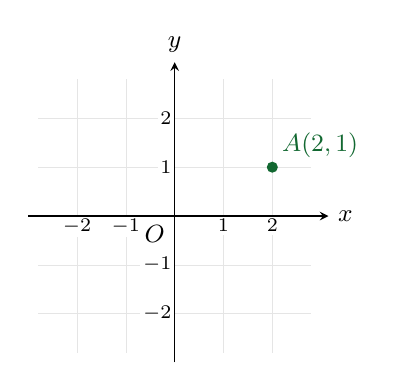
\begin{tikzpicture}[x=.62cm,y=.62cm,>=stealth,font=\small]
\draw[step=1,gray!20,very thin] (-2.8,-2.8) grid (2.8,2.8);
\draw[->] (-3,0)--(3.15,0) node[right]{$x$};
\draw[->] (0,-3)--(0,3.15) node[above]{$y$};
\node[below left] at (0,0){$O$};
\foreach \t in {-2,-1,1,2}{\node[below,fill=white,inner sep=1pt] at (\t,0){\scriptsize $\t$};\node[left,fill=white,inner sep=1pt] at (0,\t){\scriptsize $\t$};}
\fill[campusgreen] (2,1) circle(2pt) node[above right]{$A(2,1)$};\end{tikzpicture}\end{minipage}\hfill\begin{minipage}{.52\linewidth}\vspace*{4cm}\end{minipage}
\vfill{\small 本课自编练习。第1页，共2页。}
\newpage
\noindent\textbf{5. 检查下面的计算，指出最早出错的等号，并改正。}
\[i(3-2i)=3i-2i^2=-2+3i.\]
\par\vspace*{2.4cm}
\noindent\textbf{6. 独立完成。}
\par （1）计算$i(2-i)$，写出结果对应的点。
\par （2）用一句话说明：乘以$i$，图形上发生了什么？
\par （3）如果得到$-1+2i$，应重新检查哪一步？
\par\vspace*{2.4cm}
\noindent\textbf{7. 记录今天的一次理解变化。}
\par 写出自己原先不理解的一点、怎样检查或修正，以及现在能独立说明的内容。可以结合旋转问题、正方形问题或课堂中的一次计算。
\par\vspace*{2.4cm}
\vfill{\small 本课自编练习。第2页，共2页。}
\end{document}
